
%(BEGIN_QUESTION)
% Copyright 2011, Tony R. Kuphaldt, released under the Creative Commons Attribution License (v 1.0)
% This means you may do almost anything with this work of mine, so long as you give me proper credit

An electronic DP transmitter has an input range of 0 to 100 inches water column and an output range of 4 to 20 mA.  When subjected to a 5-step up-and-down ``As-Found'' calibration test, it responds as such: 

% No blank lines allowed between lines of an \halign structure!
% I use comments (%) instead, so that TeX doesn't choke.

$$\vbox{\offinterlineskip
\halign{\strut
\vrule \quad\hfil # \ \hfil & 
\vrule \quad\hfil # \ \hfil \vrule \cr
\noalign{\hrule}
%
% First row
Applied pressure & Output signal \cr
%
% Another row
(" WC) & (mA) \cr
%
\noalign{\hrule}
%
% Another row
0 & 4.0 \cr
%
\noalign{\hrule}
%
% Another row
25 & 8.7 \cr
%
\noalign{\hrule}
%
% Another row
50 & 12.8 \cr
%
\noalign{\hrule}
%
% Another row
75 & 16.6 \cr
%
\noalign{\hrule}
%
% Another row
100 & 20.0 \cr
%
\noalign{\hrule}
%
% Another row
75 & 16.6 \cr
%
\noalign{\hrule}
%
% Another row
50 & 12.8 \cr
%
\noalign{\hrule}
%
% Another row
25 & 8.7 \cr
%
\noalign{\hrule}
%
% Another row
0 & 4.0 \cr
%
\noalign{\hrule}
} % End of \halign 
}$$ % End of \vbox

Graph this instrument's ideal transfer function on the graph below, along with its {\it actual} transfer function graph based on the measured values recorded above.  Then, determine what kind of calibration error it has ({\it zero shift}, {\it span shift}, and/or {\it linearity}).

$$\includegraphics[width=15.5cm]{i03859x01.eps}$$

Hint: a computer spreadsheet program might be a useful tool in graphing this instrument's response.  Feel free to attach a printed copy of a spreadsheet graph instead of hand-sketching one on this page.

\underbar{file i03859}
%(END_QUESTION)





%(BEGIN_ANSWER)


%(END_ANSWER)





%(BEGIN_NOTES)

This transmitter definitely has a {\it linearity} error:

$$\includegraphics[width=15.5cm]{i03859x02.eps}$$

%INDEX% Calibration errors, identifying

%(END_NOTES)

